\section{Auswertung}
\label{sec:Auswertung}

\subsection{Vorbereitung}
Die gemessenen Werte sind absolute Positionen auf der Messschiene. Der reale Abstand zum Bilderzeuger ist also die Differenz zwischen der Position des entsprechenden optischen Objektes
und der Position der Schablone. Für alle Messreihen ist die Schablonenposition sowie -größe konstant. Die Schablonenhöhe wird von dem obersten zum untersten Punkt der langen Kante gemessen.

\begin{table}
    \centering
    \caption{Allgemeine Randdaten.}
    \begin{tabular}{c c}
        \toprule
        {Ursprung $U \:/\: \si{\centi\meter}$} & Höhe der Schablone $l \:/\: \si{\centi\meter}$\\
        \midrule
        29.4 & 3 \\
    \end{tabular}
    \label{tab:rand}
\end{table}

Die einzelnen Abstände berechnen sich wie in den folgenden Gleichungen.

\begin{equation}
    \begin{gathered}
        g_i = |U - L_i| \\
        b_i = |S_i - L_i| \\
        e_i = |U - S_i|
    \end{gathered}
    \label{eqn:abstand}
\end{equation}
Hierbei sind $S_i$ und $L_i$ die Messgrößen für die absoluten Positionen des Schirms und der Linse.

\subsection{Auswertung -- Einfache Messreihe}
Die sich aus den Messdaten errechneten Werte für $g_i$, $b_i$ und $f_i$ sind in Tabelle \ref{tab:mess1} festgehalten.

\begin{table}
    \centering
    \caption{Messwerte der ersten Messreihe.}
    \begin{tabular}{c c c c c}
        \toprule
        {$S_i \:/\: \si{\centi\meter}$} & {$L_i \:/\: \si{\centi\meter}$} & {$g_i \:/\: \si{\centi\meter}$} & {$b_i \:/\: \si{\centi\meter}$} & {$f_i \:/\: \si{\centi\meter}$}\\
        \midrule
        100.0    & 74.4 & 45.0 & 25.6 & 16.32 \\
        103.5    & 79.1 & 49.7 & 24.4 & 16.37 \\
        94.4     & 60.9 & 31.5 & 33.5 & 16.23 \\
        114.6    & 92.6 & 63.2 & 22.0 & 16.32 \\
        110.5    & 88.1 & 58.7 & 22.4 & 16.21 \\
        104.2    & 80.2 & 50.8 & 24.0 & 16.30 \\
        97.1     & 69.7 & 40.3 & 27.4 & 16.31 \\
        95.9     & 58.2 & 28.8 & 37.7 & 16.33 \\
        117.9    & 51.2 & 21.8 & 66.7 & 16.43 \\
    \end{tabular}
    \label{tab:mess1}
\end{table}

Daraus ergibt sich eine Brennweite von $f = \SI{16.31\pm0.06}{\centi\meter}$ mit einer relativen Messunsicherheit von etwa $0.4\%$.
Die reale Brennweite der Linse beträgt laut Herstellerangabe $f_H = \SI{15}{\centi\meter}$. Somit ergibt sich eine Abweichung von etwa $8.7\%$ zum Realwert.

\begin{figure}
    \centering
    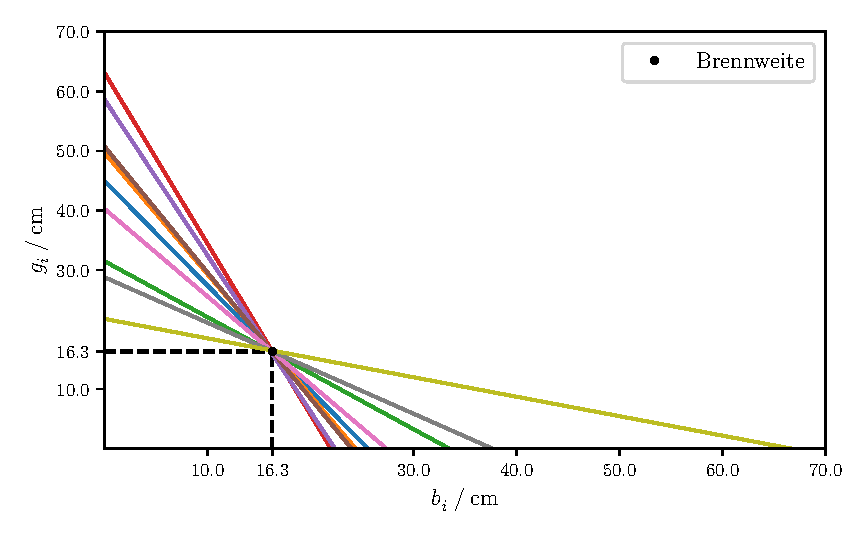
\includegraphics[width=.9\textwidth]{python/plot1.pdf}
    \caption{Graphische Darstellung der ersten Messreihe.}
    \label{fig:fokus}
\end{figure}
In der Abbildung \ref{fig:fokus} sind die Wertepaare $(g_i, b_i)$ graphisch gegeinander aufgetragen. Der gemeinsame Schnittpunkt entspricht dem für die Brennweite berechnete Wert von 
$x = y = \SI{16.31}{\centi\meter}$.

\subsection{Auswertung -- Methode von Bessel}
Die mit Hilfe von \eqref{eqn:abstand} berechneten Werte sind in Tabelle \ref{tab:mess2} eingetragen. 

\begin{table}
    \centering
    \caption{Zweite Messreihe.}
    \begin{tabular}{c c c c c c c}
        \toprule
        {$S_i \:/\: \si{\centi\meter}$} & {$L_{n,i} \:/\: \si{\centi\meter}$} & {$L_{f,i} \:/\: \si{\centi\meter}$} & {$g_{n,i} \:/\: \si{\centi\meter}$} & {$b_{n,i} \:/\: \si{\centi\meter}$}   &
        {$g_{f,i} \:/\: \si{\centi\meter}$} & {$b_{f,i} \:/\: \si{\centi\meter}$} \\
        \midrule
        81.3  &  43.2 &   67.9  &  13.8 &	38.1 &	38.5 &	13.4  \\
        89.1  &  42.4 &   76.3  &  13.0 &	46.7 &	46.9 &	12.8  \\
        72.7  &  45.4 &   57.0  &  16.0 &	27.3 &	27.6 &	15.7  \\
        77.7  &  43.9 &   63.5  &  14.5 &	33.8 &	34.1 &	14.2  \\
        81.2  &  43.2 &   67.7  &  13.8 &	38.0 &	38.3 &	13.5  \\
        88.4  &  42.7 &   75.5  &  13.3 &	45.7 &	46.1 &	12.9  \\
        93.4  &  42.2 &   81.1  &  12.8 &	51.2 &	51.7 &	12.3  \\
        100   &  41.9 &   87.8  &  12.5 &	58.1 &	58.4 &	12.2  \\
        104.8 &  41.7 &   93.1  &  12.3 &	63.1 &	63.7 &	11.7  \\
    \end{tabular}
    \label{tab:mess2}
\end{table}
Die Methode von Bessel nimmt an, dass für jedes Messpaar $b_1=g_2$ und $b_2=g_1$ gilt. In der Realität sind die Werte jedoch leicht verschieden, wie die Daten in der Wertetabelle \ref{tab:mess2}
zeigen. Ein Wertepaar besteht jeweils aus $(g_n, b_n)$ für die beiden Messgrößen des nahen Fokuspunktes und $(g_f, b_f)$ für den vom Bilderzeuger entfernteren Fokuspunkt.
Daraus ergeben sich unterschiedliche Werte für die Distanz $d = |g_i - b_i|$. Der Abstand $e = |S - U|$ ist für beide Fokuspunkte konstant.
Die durch diese Methode berechneten Werte sind in Tabelle \ref{tab:bessel} gegenübergestellt.

\begin{table}
    \centering
    \caption{Berechnete Brennweiten nach Bessel.}
    \begin{tabular}{c c c c c}
        \toprule
        {$e \:/\: \si{\centi\meter}$} & {$d_{n,i} \:/\: \si{\centi\meter}$} & {$d_{f,i} \:/\: \si{\centi\meter}$} & {$f_{n,i} \:/\: \si{\centi\meter}$} & {$f_{f,i} \:/\: \si{\centi\meter}$} \\
        \midrule
        51.9 &	24.3 &	25.1 &	10.1 &	9.9   \\
        59.7 &	33.7 &	34.1 &	10.2 &	10.1  \\
        43.3 &	11.3 &	11.9 &	10.1 &	10.0  \\
        48.3 &	19.3 &	19.9 &	10.1 &	10.0  \\
        51.8 &	24.2 &	24.8 &	10.1 &	10.0  \\
        59.0 &	32.4 &	33.2 &	10.3 &	10.1  \\
        64.0 &	38.4 &	39.4 &	10.2 &	9.9   \\
        70.6 &	45.6 &	46.2 &	10.3 &	10.1  \\
        75.4 &	50.8 &	52.0 &	10.3 &	9.9   \\
    \end{tabular}
    \label{tab:bessel}
\end{table}
Für die nahen und fernen Fokuspunkte ergeben sich somit die Brennweiten $f_n = \SI{10.20\pm0.08}{\centi\meter}$ und $f_f = \SI{10.00\pm0.07}{\centi\meter}$.
Zusammen ergibt das eine Brennweite von $f = \SI{10.10\pm0.05}{\centi\meter}$. Die relative Messunsicherheit beträgt $0.5\%$.
Die Herstellerangabe der verwendeten Linse ist $f_H = \SI{10}{\centi\meter}$. Damit beträgt die Abweichung etwa $1\%$.

\subsection{Auswertung -- Methode von Abbe}
In der Methode nach Abbe werden die Brennweite und die Lage der Hauptebenen durch eine lineare Regression bestimmt (\texttt{numpy.polyfit}\cite{numpy}). Die durch 
\begin{equation}
    \begin{gathered}
        g' = |A - U|    \\
        b' = |S - A|    \\
        V = \frac{l_i}{l}
    \end{gathered}
\end{equation}
bestimmten Werte werden mit $(1+\sfrac{1}{V},g')$ und $(1+V,b')$ je gegeneinander aufgetragen. Der dazugehörige Datensatz wird in Tabelle \ref{tab:mess3} gezeigt.

\begin{table}
    \centering
    \caption{Messwerte der dritten Messreihe.}
    \begin{tabular}{c c c c c c c}
        \toprule
        {$S_i \:/\: \si{\centi\meter}$} & {$A \:/\: \si{\centi\meter}$} & {$g_i' \:/\: \si{\centi\meter}$} & {$b_i' \:/\: \si{\centi\meter}$} 
        & {$(1+\sfrac{1}{V}) \:/\: \si{\centi\meter}$} & {$(1+V) \:/\: \si{\centi\meter}$} & {$l_i \:/\: \si{\centi\meter}$}\\
        \midrule
        119.7 &  67.3 & 37.9 &	52.5 &	2.2 & 1.8 & 2.5 \\
        135.2 &  51.5 & 22.1 &	83.7 &	1.4 & 3.2 & 6.7 \\
        118.3 &  59.7 & 30.3 &	58.6 &	1.9 & 2.2 & 3.5 \\
        119.0 &  71.1 & 41.7 &	47.9 &	2.5 & 1.7 & 2.0 \\
        122.3 &  75.5 & 46.1 &	46.8 &	2.9 & 1.5 & 1.6 \\
        117.4 &  65.2 & 35.8 &	52.2 &	2.2 & 1.8 & 2.5 \\
        125.8 &  83.1 & 53.7 &	42.7 &	3.1 & 1.5 & 1.4 \\
        132.1 &  90.0 & 60.6 &	42.1 &	3.3 & 1.4 & 1.3 \\
        138.6 &  97.5 & 68.1 &	41.1 &	3.7 & 1.4 & 1.1 \\
    \end{tabular}
    \label{tab:mess3}
\end{table}

\begin{figure}
    \centering
    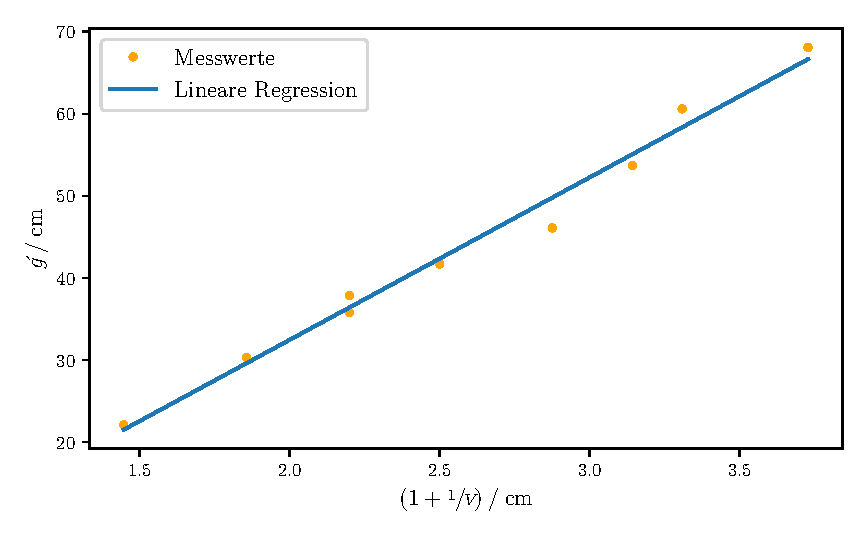
\includegraphics[width=.9\textwidth]{python/plotAbbe1.pdf}
    \caption{Messwerte und Ausgleichsgerade nach Abbe für $g_i'$}
    \label{fig:lin1}
\end{figure}

\begin{figure}
    \centering
    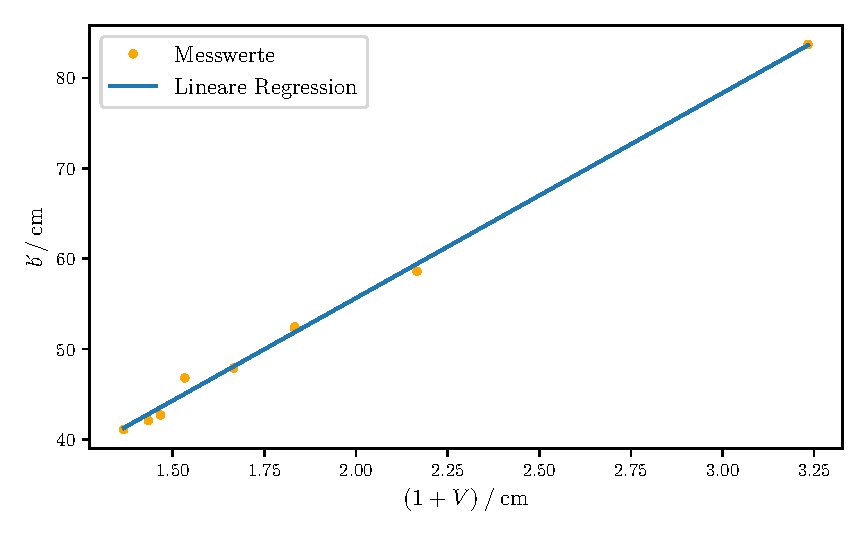
\includegraphics[width=.9\textwidth]{python/plotAbbe2.pdf}
    \caption{Messwerte und Ausgleichsgerade nach Abbe für $b_i'$}
    \label{fig:lin2}
\end{figure}

Für die Hauptebene $H$ berechnet sich aus der linearen Regression eine Brennweite von $f_1 = \SI{19.8\pm0.9}{\centi\meter}$ und eine Position von $h = \SI{-7.2\pm2.5}{\centi\meter}$.
Analog ergibt sich für die Hauptebene $H'$ eine Brennweite $f_2 = \SI{22.7\pm0.5}{\centi\meter}$ und eine Position von $h' = \SI{10.3\pm1.0}{\centi\meter}$.
Die Brennweiten haben relative Messunsicherheiten von je $f_{1, rel} = 5\%$ und $f_{2, rel} = 2\%$. Daraus ergibt sich eine gemeinsame Brennweite von 
$f = \SI{21.2\pm0.5}{\centi\meter}$ mit einer relativen Messunsicherheit von etwa $2\%$.
Für die Hauptebenen zeigen sich relative Unsicherheiten von je $35\%$ und $9.8\%$.
Die Herstellerangaben der Linsen sind $\SI{10}{\centi\meter}$ für die Sammellinse und $\SI{-10}{\centi\meter}$ für die Zerstreuungslinse. Damit haben die errechneten Werte eine Abweichung
von ungefähr $6\%$ vom Realwert.